% pcm_forward_model_slides_with_actual_images.tex
\documentclass[aspectratio=169]{beamer}

\usetheme{Madrid}
\usecolortheme{default}

\usepackage{amsmath,amssymb,bm}
\usepackage{tikz}
\usetikzlibrary{arrows.meta,positioning,calc}

\newcommand{\one}{\mathbf{1}}
\newcommand{\R}{\mathbb{R}}

% --- TikZ helpers (small grid images) ---
\tikzset{
  pix/.style={draw=black!35, line width=0.15pt},
  box/.style={draw=black!60, rounded corners, inner sep=3pt},
  arrow/.style={-{Stealth[length=2.2mm]}, line width=0.5pt},
}

% Binary mask b: 1 in top-left quadrant, 0 elsewhere (8x8)
\newcommand{\BinaryMaskEight}{
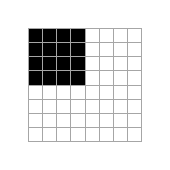
\begin{tikzpicture}[x=0.18cm,y=0.18cm]
  % frame
  \draw[black!60, line width=0.35pt] (0,0) rectangle (8,8);
  % cells
  \foreach \i in {0,...,7}{
    \foreach \j in {0,...,7}{
      \ifnum\i<4\relax
        \ifnum\j>3\relax
          \fill[black] (\i,\j) rectangle ++(1,1);
        \else
          \fill[white] (\i,\j) rectangle ++(1,1);
        \fi
      \else
        \fill[white] (\i,\j) rectangle ++(1,1);
      \fi
      \draw[pix] (\i,\j) rectangle ++(1,1);
    }
  }
\end{tikzpicture}
}

% Complementary mask \bar b = 1-b (8x8)
\newcommand{\BinaryMaskComplementEight}{
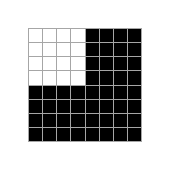
\begin{tikzpicture}[x=0.18cm,y=0.18cm]
  \draw[black!60, line width=0.35pt] (0,0) rectangle (8,8);
  \foreach \i in {0,...,7}{
    \foreach \j in {0,...,7}{
      \ifnum\i<4\relax
        \ifnum\j>3\relax
          \fill[white] (\i,\j) rectangle ++(1,1);
        \else
          \fill[black] (\i,\j) rectangle ++(1,1);
        \fi
      \else
        \fill[black] (\i,\j) rectangle ++(1,1);
      \fi
      \draw[pix] (\i,\j) rectangle ++(1,1);
    }
  }
\end{tikzpicture}
}

% Signed pattern h = 2b - 1 (8x8): +1 = black, -1 = gray
\newcommand{\SignedPatternEight}{
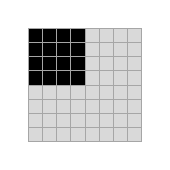
\begin{tikzpicture}[x=0.18cm,y=0.18cm]
  \draw[black!60, line width=0.35pt] (0,0) rectangle (8,8);
  \foreach \i in {0,...,7}{
    \foreach \j in {0,...,7}{
      \ifnum\i<4\relax
        \ifnum\j>3\relax
          \fill[black] (\i,\j) rectangle ++(1,1); % +1
        \else
          \fill[black!15] (\i,\j) rectangle ++(1,1); % -1
        \fi
      \else
        \fill[black!15] (\i,\j) rectangle ++(1,1); % -1
      \fi
      \draw[pix] (\i,\j) rectangle ++(1,1);
    }
  }
\end{tikzpicture}
}

% Hadamard-like illustrative patterns (8x8): DC, half/half, checkerboard
\newcommand{\PatternDC}{
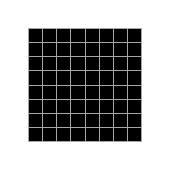
\begin{tikzpicture}[x=0.18cm,y=0.18cm]
  \draw[black!60, line width=0.35pt] (0,0) rectangle (8,8);
  \foreach \i in {0,...,7}{
    \foreach \j in {0,...,7}{
      \fill[black] (\i,\j) rectangle ++(1,1);
      \draw[pix] (\i,\j) rectangle ++(1,1);
    }
  }
\end{tikzpicture}
}
\newcommand{\PatternHalf}{
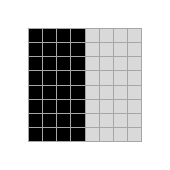
\begin{tikzpicture}[x=0.18cm,y=0.18cm]
  \draw[black!60, line width=0.35pt] (0,0) rectangle (8,8);
  \foreach \i in {0,...,7}{
    \foreach \j in {0,...,7}{
      \ifnum\i<4\relax
        \fill[black] (\i,\j) rectangle ++(1,1);
      \else
        \fill[black!15] (\i,\j) rectangle ++(1,1);
      \fi
      \draw[pix] (\i,\j) rectangle ++(1,1);
    }
  }
\end{tikzpicture}
}
\newcommand{\PatternChecker}{
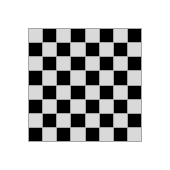
\begin{tikzpicture}[x=0.18cm,y=0.18cm]
  \draw[black!60, line width=0.35pt] (0,0) rectangle (8,8);
  \foreach \i in {0,...,7}{
    \foreach \j in {0,...,7}{
      \pgfmathtruncatemacro{\p}{mod(\i+\j,2)}
      \ifnum\p=0\relax
        \fill[black] (\i,\j) rectangle ++(1,1);
      \else
        \fill[black!15] (\i,\j) rectangle ++(1,1);
      \fi
      \draw[pix] (\i,\j) rectangle ++(1,1);
    }
  }
\end{tikzpicture}
}

\title{PCM Forward Model}
\subtitle{Consistent notation with illustrative diagrams}
\author{}
\date{}

\begin{document}

\begin{frame}
  \titlepage
\end{frame}

% --- Slide 1: pipeline graphic ---
\begin{frame}{Forward model overview (one consistent notation)}
\begin{columns}[T,onlytextwidth]
  \begin{column}{0.58\textwidth}
    \begin{itemize}
      \item Unknown current map (vectorised image): \(x \in \R^n\).
      \item Binary masks \(b_m \in \{0,1\}^n\) shown on the DMD.
      \item Differential measurement yields a signed pattern \(h_m = 2b_m-\one \in \{\pm1\}^n\).
      \item Stack rows into \(H \in \{\pm1\}^{M\times n}\):
      \[
        y = Hx + e.
      \]
    \end{itemize}
  \end{column}
  \begin{column}{0.42\textwidth}
    \centering
    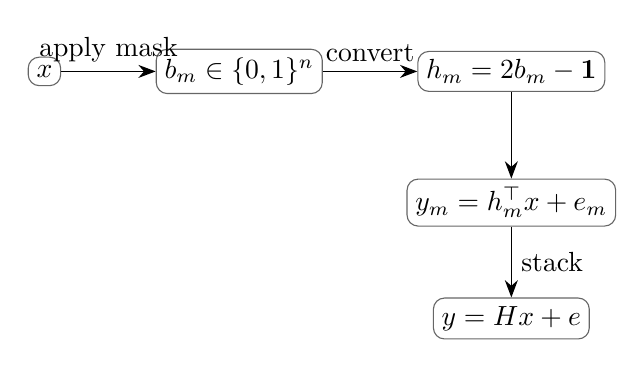
\begin{tikzpicture}[node distance=1.0em]
      \node[box] (x) {\(x\)};
      \node[box, right=1.2cm of x] (b) {\(b_m \in \{0,1\}^n\)};
      \node[box, right=1.2cm of b] (h) {\(h_m = 2b_m-\one\)};
      \node[box, below=1.1cm of h] (y) {\(y_m = h_m^\top x + e_m\)};
      \node[box, below=0.9cm of y] (Y) {\(y = Hx + e\)};

      \draw[arrow] (x) -- node[above]{apply mask} (b);
      \draw[arrow] (b) -- node[above]{convert} (h);
      \draw[arrow] (h) -- (y);
      \draw[arrow] (y) -- node[right]{stack} (Y);
    \end{tikzpicture}
  \end{column}
\end{columns}
\end{frame}

% --- Slide 2: vectorisation image ---
\begin{frame}{Vectorising the image: 2D map \(\to\) \(x \in \R^n\)}
\begin{columns}[T,onlytextwidth]
  \begin{column}{0.60\textwidth}
    \begin{itemize}
      \item Treat the 2D current map as a vector \(x\) by stacking pixels.
      \item Masks and Hadamard patterns act on the vectorised form.
    \end{itemize}
    \[
      x \in \R^n,\quad n = N_{\mathrm{pix}} = N_x N_y.
    \]
  \end{column}
  \begin{column}{0.40\textwidth}
    \centering
    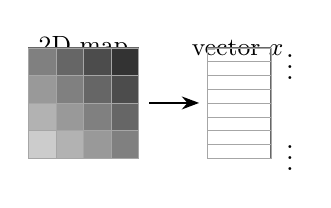
\begin{tikzpicture}[x=0.35cm,y=0.35cm]
      % small 4x4 image
      \node at (2,5.0) {\small 2D map};
      \draw[black!60] (0,1) rectangle (4,5);
      \foreach \i in {0,...,3}{
        \foreach \j in {0,...,3}{
          \pgfmathtruncatemacro{\v}{10*(\i+\j)+20}
          \fill[black!\v] (\i,1+\j) rectangle ++(1,1);
          \draw[pix] (\i,1+\j) rectangle ++(1,1);
        }
      }

      % arrow
      \draw[arrow] (4.4,3.0) -- (6.2,3.0);

      % vector
      \node at (7.6,5.0) {\small vector \(x\)};
      \draw[black!60] (6.5,1.0) rectangle (8.8,5.0);
      \foreach \k in {0,...,7}{
        \draw[pix] (6.5,1.0+0.5*\k) rectangle ++(2.3,0.5);
      }
      \node[anchor=west] at (9.0,4.6) {\(\vdots\)};
      \node[anchor=west] at (9.0,1.3) {\(\vdots\)};
    \end{tikzpicture}
  \end{column}
\end{columns}
\end{frame}

% --- Slide 3: masks and signed pattern images ---
\begin{frame}{Complementary masks and the signed pattern}
\begin{columns}[T,onlytextwidth]
  \begin{column}{0.58\textwidth}
    \[
    \begin{aligned}
    y_m^{+} &= \langle b_m, x\rangle + \eta_m^{+},\\
    y_m^{-} &= \langle \one-b_m, x\rangle + \eta_m^{-},\\
    y_m &:= y_m^{+}-y_m^{-} = \langle 2b_m-\one, x\rangle + e_m
         = h_m^\top x + e_m.
    \end{aligned}
    \]
    \[
      h_m := 2b_m-\one,\quad e_m := \eta_m^{+}-\eta_m^{-}.
    \]
  \end{column}
  \begin{column}{0.42\textwidth}
    \centering
    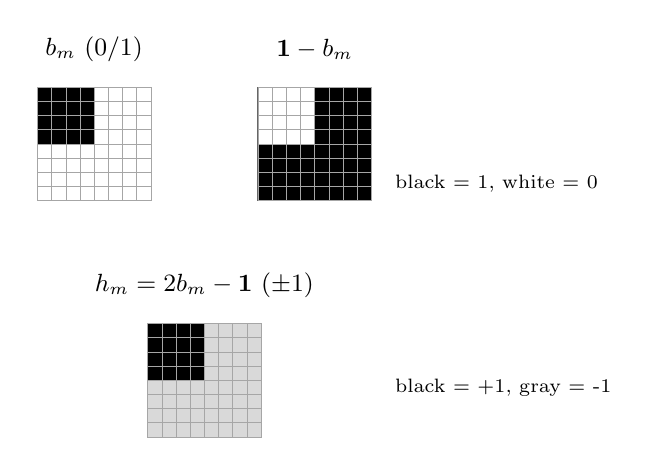
\begin{tikzpicture}
      \node at (0,2.1) {\small \(b_m\) (0/1)};
      \node at (2.8,2.1) {\small \(\one-b_m\)};
      \node at (1.4,-0.9) {\small \(h_m=2b_m-\one\) (\(\pm1\))};

      \node at (0,0.9) {\BinaryMaskEight};
      \node at (2.8,0.9) {\BinaryMaskComplementEight};
      \node at (1.4,-2.1) {\SignedPatternEight};

      \node[anchor=west] at (3.7,-2.2) {\scriptsize black = +1, gray = -1};
      \node[anchor=west] at (3.7,0.4) {\scriptsize black = 1, white = 0};
    \end{tikzpicture}
  \end{column}
\end{columns}
\end{frame}

% --- Slide 4: coarse-to-fine patterns image + subsampling diagram ---
\begin{frame}{Walsh-Hadamard patterns and subsampling}
\begin{columns}[T,onlytextwidth]
  \begin{column}{0.58\textwidth}
    Full basis (unnormalised):
    \[
      W \in \{\pm1\}^{n\times n},\qquad W^\top W = nI.
    \]
    Subsampling as row-selection:
    \[
      H = SW,\qquad S \in \{0,1\}^{M\times n}.
    \]
    Coarse-to-fine ordering: select low-frequency patterns first (illustrated).
  \end{column}
  \begin{column}{0.42\textwidth}
    \centering
    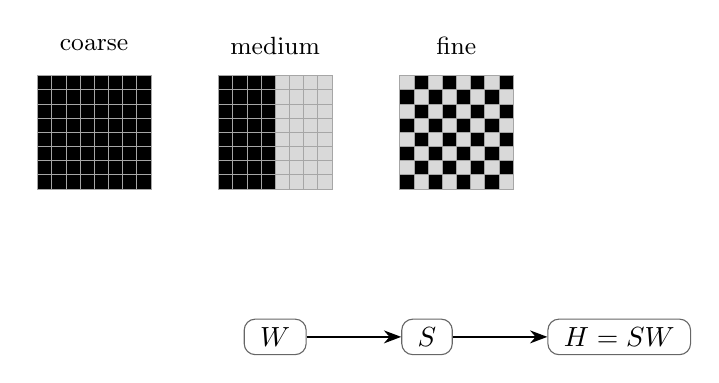
\begin{tikzpicture}[node distance=0.6em]
      \node at (1.2,2.0) {\small coarse};
      \node at (3.5,2.0) {\small medium};
      \node at (5.8,2.0) {\small fine};

      \node at (1.2,0.9) {\PatternDC};
      \node at (3.5,0.9) {\PatternHalf};
      \node at (5.8,0.9) {\PatternChecker};

      \node[box] (W) at (3.5,-1.7) {\(\;W\;\)};
      \node[box, right=1.2cm of W] (S) {\(\;S\;\)};
      \node[box, right=1.2cm of S] (H) {\(\;H=SW\;\)};
      \draw[arrow] (W) -- (S);
      \draw[arrow] (S) -- (H);
    \end{tikzpicture}
  \end{column}
\end{columns}
\end{frame}

% --- Slide 5: inversion / zero-filled pipeline image ---
\begin{frame}{Inverse WHT (full sampling) and zero-filled backprojection (subsampling)}
\begin{columns}[T,onlytextwidth]
  \begin{column}{0.60\textwidth}
    Unnormalised convention (\(W^\top W = nI\)):

    \[
      \text{Full sampling }(M=n,\, H=W):\quad x = \frac{1}{n}W^\top y.
    \]

    \[
      \text{Subsampling }(y=SWx+e):\quad
      \hat x_{\mathrm{zf}} = \frac{1}{n}W^\top S^\top y.
    \]

    Normalised convention \(\tilde W = \frac{1}{\sqrt{n}}W\) removes the factor \(1/n\).
  \end{column}
  \begin{column}{0.40\textwidth}
    \centering
    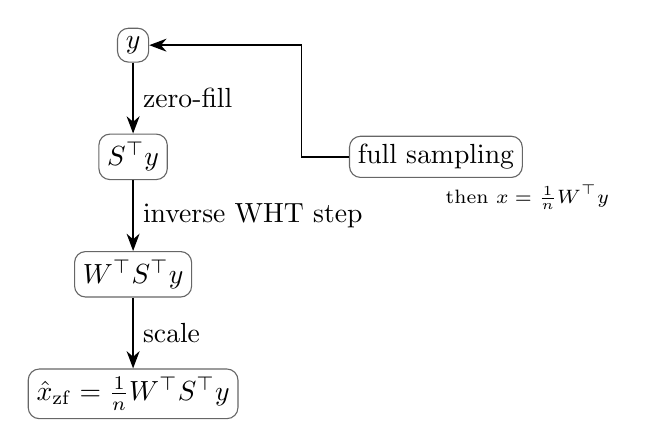
\begin{tikzpicture}[node distance=0.9em]
      \node[box] (y) {\(y\)};
      \node[box, below=0.9cm of y] (St) {\(S^\top y\)};
      \node[box, below=0.9cm of St] (Wt) {\(W^\top S^\top y\)};
      \node[box, below=0.9cm of Wt] (xhat) {\(\hat x_{\mathrm{zf}} = \frac{1}{n}W^\top S^\top y\)};

      \draw[arrow] (y) -- node[right]{zero-fill} (St);
      \draw[arrow] (St) -- node[right]{inverse WHT step} (Wt);
      \draw[arrow] (Wt) -- node[right]{scale} (xhat);

      \node[box, right=2.3cm of St] (full) {full sampling};
      \draw[arrow] (full.west) -- ++(-0.6,0) |- (y.east);
      \node[anchor=west] at ($(full.south)+(0,-0.25)$) {\scriptsize then \(x=\frac{1}{n}W^\top y\)};
    \end{tikzpicture}
  \end{column}
\end{columns}
\end{frame}

\end{document}
